\setchapterpreamble[u]{\margintoc} 
\chapter{Évaluer les performances d'un SLCI} 
\section{Évaluer la stabilité en utilisant la BF, les pôles de la BF} 
\section{Évaluer la stabilité en utilisant les marges de la BO} 
\graphicspath{{\repStyle/png/}{../PERF/PERF-02-Marges/61_Hemostase/images/}} 
\normaltrue
\correctionfalse

%\UPSTIidClasse{12} % 11 sup, 12 spé
%\newcommand{\UPSTIidClasse}{12}

\exer{Automate d’exploration de l’hémostase $\star$ \label{C2:091D:61}}
\setcounter{question}{0}\UPSTIcompetence[2]{C2-09}
\index{Compétence C2-09}
\index{Principe fondamental de la dynamique}
\index{PFD}
%\index{Mécanisme à 1 rotation}
\index{Automate d’exploration de l’hémostase}
\ifcorrection
\else
\marginnote{\textbf{Pas de corrigé pour cet exercice.}}
\fi

\ifprof
\else
Afin de valider le choix des moteurs, on étudie le déplacement sur l’axe $\vect{x}$.% qui est le plus grand. 
On note $V_x$ la vitesse selon cet axe.
On rappelle que la distance maximum à parcourir est $x_M^{\text{max}} = \SI{550}{mm}$ en 1 seconde.
La loi de commande sur chaque axe est définie par un trapèze de vitesse (\autoref{61_01})
avec les temps d’accélération et de décélération ($T_a$) identiques. De plus, les moteurs se mettent en route et s’arrêtent en
même temps. $T$ est la durée totale du déplacement. Nous allons chercher à optimiser cette loi de commande de sorte
que le moteur fournisse une puissance instantanée minimale.

\begin{figure}[H]
\centering
\includegraphics[width=.8\linewidth]{61_01}
\caption{\label{61_01} Loi de commande de vitesse en trapèze}
\end{figure}

Le modèle de calcul pour cette commande d’axe est le suivant :
\begin{itemize}
\item le mouvement de rotation du moteur (vitesse $\omega_m^x$) est transformé en mouvement de translation (vitesse $V^x$) ;
\item le rapport de transmission de la chaîne cinématique est $\lambda = \dfrac{V^x}{\omega_m^x}$;
\item la distance à parcourir est $x_M^{\text{max}}$;
\item l’inertie équivalente de l’ensemble des pièces en mouvement ramenée à l’arbre moteur est $J_e$;
\item les frottements et la pesanteur sont négligés, il n’y a donc pas de couple résistant.
\end{itemize}
\fi
\question{Exprimer la vitesse maximale $V_M^x$ en fonction de $x_M^{\text{max}}$, $T$ et $T_a$.}
\ifprof
La distance  $x_M^{\text{max}}$ correspond à l'aire sous le courbe de la loi de commande de vitesse.
On a alors 
 $x_M^{\text{max}} = \left(T-T_a\right)V_M^x$ 
 $ \Longleftrightarrow V_M^x=\dfrac{x_M^{\text{max}}}{T-T_a}$. 
\else
\fi

\question{Par application du théorème de l’énergie cinétique sur l’ensemble des pièces en mouvement,
exprimer le couple moteur $C_m$ en fonction de $V_x$, $T_a$, $J_e$ et $\lambda$ durant les trois phases du
mouvement.}
\ifprof
\begin{itemize}
\item Expression de l'énerige cinétique : $\ec{E}{0}=\dfrac{1}{2}J_e (\omega_m^x)^2$.
\item Puissance intérieure : $\mathcal{P}_{\text{int}}(E)=0$.
\item Puissance extérieure : $\mathcal{P}_{\text{ext}}(E)=C_m\omega_m^x$.
\item Application du TEC : $J_e \omega_m^x \dot{\omega}_m^x = C_m\omega_m^x$ soit $J_e  \dot{\omega}_m^x = C_m$.
\end{itemize}
\vspace{.25cm}

On a alors sur chacune des phases : 

\begin{itemize}
\item Phase 1 : $C_m=J_e  \dot{\omega}_m^x$ avec $\dot{\omega}_m^x = \dot{V_M}^x /  \lambda= \dfrac{V_M^x}{ \lambda T_a}$ et $C_m = J_e \dfrac{V_M^x}{\lambda T_a}$.
\item Phase 2 : $C_m=0$.
\item Phase 3 : $C_m = - J_e  \dfrac{V_M^x}{\lambda T_a}$.
\end{itemize}

\else
\fi

\question{Préciser à quel(s) instant(s) $t$ la puissance fournie par le moteur est maximale ($P_{\text{max}}$)}.
\ifprof
\else
\fi

\question{Exprimer cette puissance $P_{\text{max}}$ en fonction de $V_M^x$, $\lambda$, $J_e$, et $T_a$.}
\ifprof
$P_{\text{max}} = J_e \dfrac{V_M^x}{\lambda T_a}  {\omega}_m^x =J_e \dfrac{(V_M^x)^2}{\lambda^2 T_a}$.
\else
\fi

\question{Donner alors l’expression de $P_{\text{max}}$ en fonction de $x_M^{\text{max}}$, $\lambda$, $J_e$, et $T_a$.}
\ifprof
On a alors 
$P_{\text{max}} =J_e \dfrac{\left({x_M^{\text{max}}}\right)^2}{\lambda^2 \left({T-T_a}\right)^2 T_a}$.
\else
\fi

\question{À partir de cette expression, montrer que $P_{\text{max}}$ est minimale pour un réglage du
temps d’accélération $T_a$ tel que $T_a=\dfrac{T}{3}$.}
\ifprof
On résout $\dfrac{\dd P_{\text{max}}}{\dd T_a} = 0$ et on cherche la valeur de $T_a$ pour laquelle 
$P_{\text{max}}$ est minimale.

\else
\fi

\ifprof
\else
Pour cette nouvelle commande avec $T_a=\dfrac{T}{3}$, on cherche à valider le choix du moteur en étudiant le
déplacement maximum suivant $\vect{x}$. Les caractéristiques de la chaîne cinématique sont :
\begin{itemize}
\item vitesse maximale du moteur : $N_{\text{max}}^{\text{mot}}=\SI{4150}{tr.min^{-1}}$;
\item rapport de réduction du réducteur $k=\dfrac{1}{10}$;
\item rayon de poulie $R_p= \SI{20}{mm}$.
\end{itemize}
\fi

\question{Déterminer la vitesse de rotation maximum $\omega^x_{\text{max}}$ que doit atteindre le moteur. Le
choix de celui-ci est-il validé ?}
\ifprof
On a  $V_M^x=\dfrac{x_M^{\text{max}}}{T-T_a}$. D'autre part, 
$V_M^x = \omega_M^x  k R_p $ soit $\omega_M^x  = \dfrac{V_M^x}{ k R_p} =  \dfrac{{x_M^{\text{max}}}}{ k R_p\left({T-T_a} \right)} $.

AN : $\omega_M^x  = \dfrac{550\times 10^{-3}}{ 0,1 \times 20 \times 10^{-3} \left(1-1/3 \right)} $
$ =  \dfrac{550\times 3}{ 4}= \SI{412,5}{rad.s^{-1}} $ soit \SI{3941}{tr.min^{-1}}.

Cette valeur est bien compatible avec la vitesse du moteur.
\else
\fi


\ifprof
\else
\begin{flushright}
\footnotesize{Corrigé  voir \ref{C2:091D:61}.}
\end{flushright}%
\fi 
 
\graphicspath{{\repStyle/png/}{../PERF/PERF-02-Marges/62_Palettisation/images/}} 
\normaltrue \difficilefalse \tdifficilefalse
\correctiontrue
%\UPSTIidClasse{11} % 11 sup, 12 spé
%\newcommand{\UPSTIidClasse}{11}

\exer{Palettisation -- Stabilité $\star$ \label{C2:03:stab:62}}
%% CCP MP 2010
\setcounter{question}{0}\UPSTIcompetence[2]{C2-03}
\index{Compétence C2-03}
\index{Schéma-blocs}
\index{Stabilité}

\ifcorrection
\else
\marginnote{\textbf{Pas de corrigé pour cet exercice.}}
\fi


\ifprof 
\else
Une boucle de position est représentée ci-dessous. On admet que :  
\begin{itemize}
\item $H(p)=\dfrac{\Omega_m(p)}{U_v(p)}=\dfrac{30}{1+\num{5e-3}p}$;
\item $K_r = \SI{4}{V.rad^{-1}}$ : gain du capteur de position;
\item $K_a$ : gain de l’adaptateur du signal de consigne $\alpha_e(t)$; 
\item $N=200$ : rapport de transmission du réducteur (la réduction est donc de $1/N$).
\item le signal de consigne $\alpha_e(t)$ est exprimé en degré ; 
\item le correcteur $C(p)$ est à action proportionnelle de gain réglable $K_c$. 
\end{itemize}


\begin{center}
\includegraphics[width=.9\linewidth]{62_01}
\end{center}
 \fi
 
 
 On montre que la fonction de transfert du réducteur est $R(p)=\dfrac{\alpha_r(p)}{\Omega_m(p)}=\dfrac{1}{Np}$, que  $k_a=\dfrac{\pi}{180}k_r$ et que la FTBO est donnée par $T(p)=\dfrac{k_{BO}}{p\left(1+\tau_m p\right)}$ ($k_{BO}=\dfrac{k_c k_m k_r}{N}$).
 
 
 On souhaite une marge de phase de 45\degres.
 
\question{Déterminer la valeur de $K_{BO}$ permettant de satisfaire cette condition.}
\ifprof
On souhaite une marge de phase de 45\degres. On cherche donc $\omega_{\varphi}$ tel que 
$\varphi\left(\omega_{\varphi}\right)=-180+45 = -135\degres$.

$\varphi(\omega)=-90-\arg\left(1+\tau_m j \omega \right) =-90-\arctan\left(\tau_m  \omega \right)  $.

On a donc $\varphi\left(\omega_{\varphi}\right)=-135$
$\Leftrightarrow -90-\arctan\left(\tau_m  \omega_{\varphi}\right)  = -135 $
$\Leftrightarrow -\arctan\left(\tau_m  \omega_{\varphi} \right)  = -45 $
$\Leftrightarrow \arctan\left(\tau_m  \omega_{\varphi} \right)  = 45 $
$\Rightarrow \tau_m  \omega_{\varphi} = 1 $
$\Rightarrow \omega_{\varphi}  = \dfrac{1}{\tau_m}= \dfrac{1}{5\times 10^{-3}}$
$\Rightarrow \omega_{\varphi}  = \SI{200}{rad.s^{-1}}$.


Par suite, il faut que le gain soit nul en $\omega_{\varphi}$.

On a donc $\indice{G}{dB}(\omega)=20\log k_{BO}-20\log\omega-20\log\sqrt{1+\omega^2\tau_m^2}$.
En $\omega_{\varphi} =  \dfrac{1}{\tau_m}$ :
$\indice{G}{dB}(\omega_{\varphi})=0$ 
$\Leftrightarrow 20\log k_{BO}-20\log \dfrac{1}{\tau_m}-20\log\sqrt{1+\dfrac{1}{\tau_m^2}\tau_m^2}=0$
$\Leftrightarrow \log k_{BO}+\log \tau_m-\log\sqrt{2}=0$
$\Leftrightarrow \log \dfrac{k_{BO} \tau_m}{\sqrt{2}}=0$
$\Leftrightarrow \dfrac{k_{BO} \tau_m}{\sqrt{2}}=1$
$\Leftrightarrow k_{BO}=\dfrac{\sqrt{2}}{\tau_m}$.

(\textbf{A vérifier})
$k_{BO}=282,8$.

\else 
\fi

\question{En déduire la valeur du gain $K_c$ du correcteur. }
\ifprof
$k_{BO}=\dfrac{k_c k_m k_r}{N}$; donc 
$k_c=\dfrac{Nk_{BO}}{ k_m k_r} = \dfrac{200 \times 282,8 }{4\times 30}=471$.
\else 
\fi

\question{Déterminer l’écart de position.}
\ifprof
Il y a une intégration dans la correcteur. La FTBO est de classe 1 est le système est précis en position. 
\else 
\fi

 

\ifprof
\else

\noindent\footnotesize
\fbox{\parbox{.9\linewidth}{
Éléments de corrigé : 
\begin{enumerate}
  \item $k_{BO}=\dfrac{\sqrt{2}}{\tau_m}$.
  \item $k_c=\dfrac{\sqrt{2}N}{\tau_m k_m k_r} = 471,1$.
  \item $\varepsilon_s=0$.
\end{enumerate}}}
\normalsize

\begin{flushright}
\footnotesize{Corrigé  voir \ref{C2:03:stab:62}.}
\end{flushright}%
\fi 
 
\graphicspath{{\repStyle/png/}{../PERF/PERF-02-Marges/63_BancHydraulique/images/}} 
\normaltrue
\correctionfalse

%\UPSTIidClasse{12} % 11 sup, 12 spé
%\newcommand{\UPSTIidClasse}{12}

\exer{Banc d'épreuve hydraulique $\star$ \label{C2:091D:63}}
\setcounter{question}{0}\UPSTIcompetence[2]{C2-09}
\index{Compétence C2-09}
\index{Principe fondamental de la dynamique}
\index{PFD}
%\index{Mécanisme à 1 rotation}
\index{Banc d'épreuve hydraulique} % CCP PSI 2010
\ifcorrection
\else
\marginnote{\textbf{Pas de corrigé pour cet exercice.}}
\fi

\ifprof
\else
Un schéma cinématique simplifié du chariot arrière, ainsi que les grandeurs cinématiques et cinétiques,
sont donnés figure suivante.
La chaîne de puissance comporte un moteur hydraulique, un réducteur roue et vis sans fin, un réducteur à
engrenages parallèles et un système pignon-crémaillère.
Le guidage du chariot est modélisé par une glissière.



\begin{figure}[H]
\centering
\includegraphics[width=\linewidth]{63_01}
%\caption{\label{61_01} Loi de commande de vitesse en trapèze}
\end{figure}


On note $C_m$  le couple moteur, $\omega_m$ sa vitesse de rotation par rapport au bâti, et $V$ la vitesse du chariot.
La loi de vitesse du chariot pendant la totalité du trajet est présentée ci-dessous.

\begin{figure}[H]
\centering
\includegraphics[width=\linewidth]{63_02}
%\caption{\label{61_01} Loi de commande de vitesse en trapèze}
\end{figure}


\begin{itemize}
\item On note $t_r$ la durée de la phase de déplacement rapide, $t_l$ la durée de la phase lente, $t_f$ la durée
totale, $t_a$ la durée de la phase d'accélération. Chacune des 2 phases de décélération dure $t_a/2$.
\item La course pendant la phase de déplacement en vitesse rapide (de 0 à $t_r$) est au maximum de
$c_{rap}= \SI{6,24}{m}$ (pour le tube le plus court que peut tester le banc) et pendant la phase en vitesse
lente (de $t_r$ à $t_f$) $c_{\text{lent}}= \SI{1,56}{m}$.
\item La durée maximale du déplacement total (phase rapide + phase lente) est limitée à \SI{20}{s}.
\item La vitesse du chariot, lors de la phase rapide, $V_{\text{rap}}$ est limitée à \SI{0,5}{m/s}.
\item On considérera que le module de l'accélération $a$ du chariot est identique pendant toutes les
phases d'accélération et de décélération.
\end{itemize}

\fi

\question{Exprimer $c_{\text{lent}}$ et $c_{\text{rap}}$ en fonction de $t_a$, $t_l$ et $t_r$.}
\ifprof
\else
\fi

\question{En déduire les valeurs numériques de $t_r$ et de $t_a$. En déduire l'accélération $a$ du chariot.}
\ifprof
\else
\fi

\question{Déterminer $\omega_m$ en fonction de $V$ et des données cinémtiques utiles.}
\ifprof
\else
\fi

\question{En déduire les valeurs numériques de la vitesse maximale du moteur $\omega_m$ et de l'accélération angulaire $\dot{\omega}_m$ pendant les phases d'accélération et de décélération.}
\ifprof
\else
\fi

\question{Donner l'expression de l'énergie cinétique de l'ensemble $\Sigma$ par rapport au référentiel galiléen bâti.}
\ifprof
\else
\fi

\question{En déduire l'expression de l'inertie équivalente de cet ensemble ramenée à l'axe de sortie du
moteur, notée $J_{\text{eq}}$ en fonction de $M$, $I_m$, $I_r$ et des données cinématiques utiles. Application
numérique.}
\ifprof
\else
\fi


\ifprof
\else
\begin{itemize}
\item Les efforts résistants sur le chariot sont modélisés par un glisseur $F$ d'amplitude \SI{500}{N}.
\item Le rendement de l'ensemble du mécanisme (réducteur roue et vis sans fin, réducteur à axes parallèles) est $\eta= 0,3$.
\item On prendra une accélération angulaire maximale du moteur $\dot{\omega}_m$ égale à \SI{250}{rad.s^{-2}} et une inertie totale équivalente ramenée à l'arbre moteur $J_{\text{eq}}$ égale à \SI{0,01}{kg.m^2}.
\end{itemize}
On se propose de déterminer le couple nécessaire du moteur.
\fi

\question{Déterminer l'expresion du couple $C_m$ à fournir par le moteur en fonction de $\dot{\omega}_m$, $J_{\text{eq}}$ et $F$. Calculer $C_m$.}
\ifprof
\else
\fi



\ifprof

\else
\ifcolle
\else
\footnotesize
\begin{enumerate}
 \item $c_{\text{lent}}=\dfrac{V_{\text{rap}}}{2}t_l$ et $c_{\text{rap}}=V_{\text{rap}}\left(t_r - \dfrac{1}{2}t_a\right)$.
 \item $t_a=\SI{2,56}{s}$, $t_l=\SI{6,24}{s}$, $t_r=\SI{13,76}{s}$ et $a =\SI{0,19}{m.s^{-2}}$. 
 \item $\omega_M = - \dfrac{VR_3}{rR_1R_p}$.
 \item $\omega_m = -\SI{406}{rad.s^{-1}}$ et  $\dot{\omega}_m= -\SI{158}{rad.s^{-2}}$.
 \item $\ec{\Sigma}{0} = \dfrac{1}{2}MV^2 + \dfrac{1}{2}\left( I_M + I_r \right)\omega_m^2$.
 \item $J_{\text{eq}} = I_M + I_r + M \left( \dfrac{rR_1 R_p}{R_3}\right)^2 = \SI{0,00877}{kg.m^2}$.
 \item $C_M \dfrac{J_{\text{eq}} \dot{\omega}_m + F \dfrac{rR_1R_p}{R_3}}{\eta} = \SI{10,4}{Nm}$ (rendement à voir...).
\end{enumerate}
\fi

\normalsize

\begin{flushright}
\footnotesize{Corrigé  voir \ref{C2:091D:63}.}
\end{flushright}%
\fi 
 
\graphicspath{{\repStyle/png/}{../PERF/PERF-02-Marges/64_EPAS/images/}} 
\normaltrue \difficilefalse \tdifficilefalse
\correctionfalse
%\UPSTIidClasse{11} % 11 sup, 12 spé
%\newcommand{\UPSTIidClasse}{11}

\exer{Exercice d'application $\star$ \label{PERF:02:C2:03:stab:64}}
%% CCP MP 2007
\setcounter{question}{0}\marginnote{\xpComp{PERF}{02}}%\index{Compétence C2-03}\index{Compétence PERF-02}
\index{Compétence C2-03}
\index{Schéma-blocs}
\index{Stabilite}

\ifcorrection
\else
\marginnote{\textbf{Pas de corrigé pour cet exercice.}}
\fi


\ifprof
\else
L'asservissement est donné par le schéma-blocs suivant. $H_{\text{BO}}(p) = \dfrac{4}{p\left( p+3,6\right)}$.  Le retard du système est de \SI{0,2}{s}.
De plus, $C(p)=K_c\dfrac{1+T_c p}{T_c p}$

\begin{marginfigure}
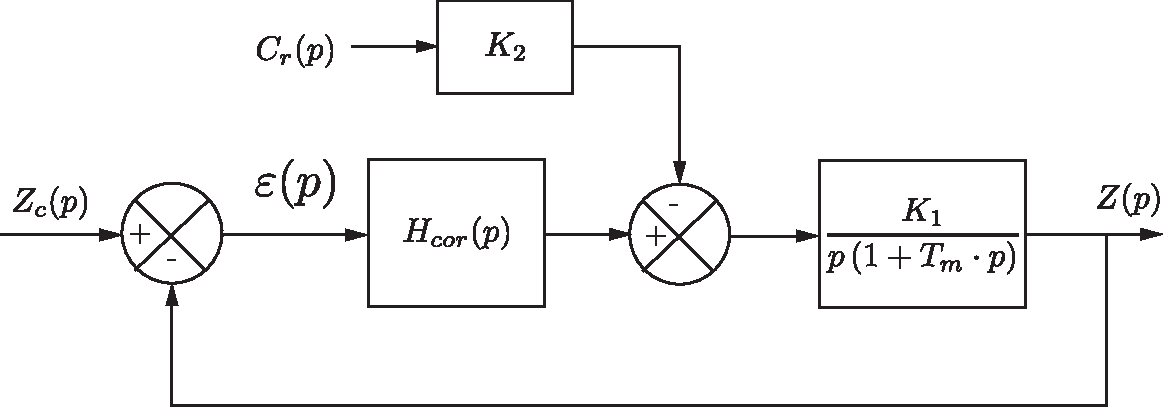
\includegraphics[width=\linewidth]{64_01}
\end{marginfigure}

\fi
 
\question{Tracer le diagramme de Bode asymptotique de $H_{\text{BO}}(p)$ pour des pulsations comprises entre \SI{0,5}{rad.s^{-1}} et \SI{50}{rad.s^{-1}}.}
\ifprof
\else 
\fi

\question{Tracer le diagramme de Bode du retard pour des pulsations comprises entre \SI{0,5}{rad.s^{-1}} et \SI{50}{rad.s^{-1}}.}
\ifprof
\else 
\fi


\ifprof
\else
On donne le diagramme de la FTBO retardée. 

\begin{marginfigure}
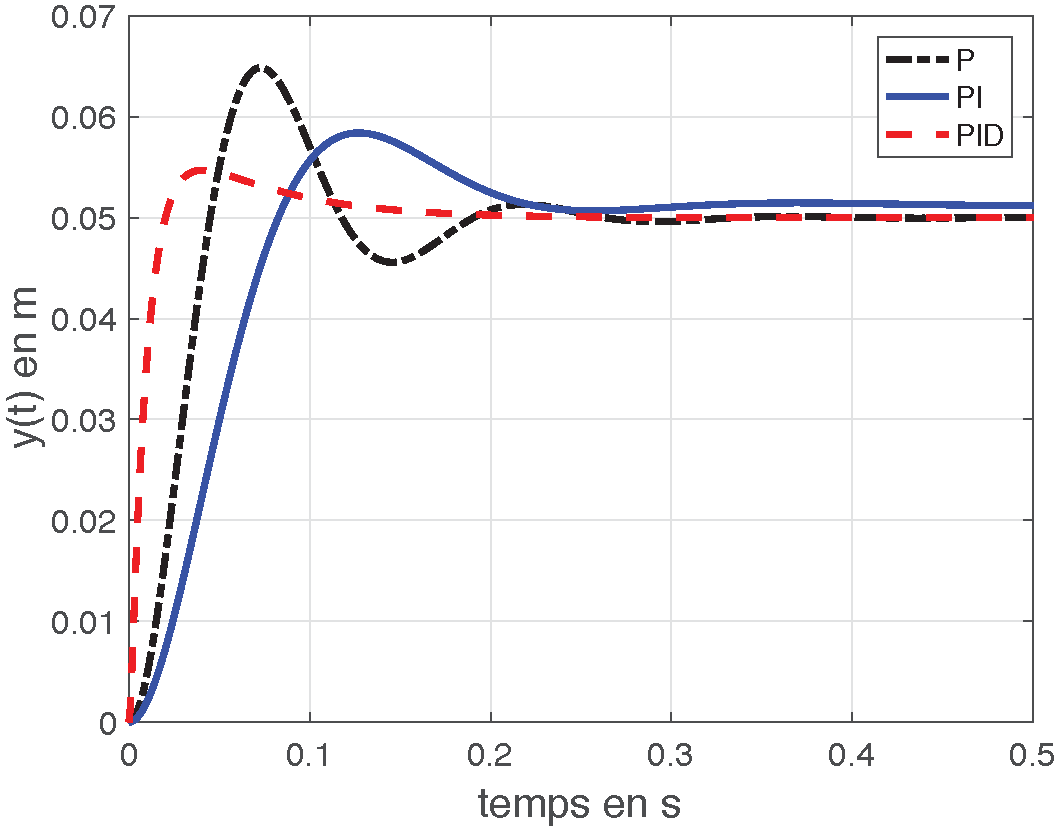
\includegraphics[width=\linewidth]{64_02}
\end{marginfigure}
\fi

\question{Déterminer le gain $K_c$ qui donne une marge de phase de 50\degres.}
\ifprof
\else 
\fi

\question{La constante $T_c$ qui laisse subsister une marge de phase d’environ 45\degres.}
\ifprof
\else 
\fi


\question{Quelle est l’erreur de traînage du système corrigé pour l’entrée en rampe considérée (en négligeant le retard).}
\ifprof
\else 
\fi


\ifprof
\else



\marginnote{Corrigé voir \ref{PERF:02:C2:03:stab:64}.}

\fi 
 
\section{Évaluer la rapidité de la réponse temporelle} 
\section{Évaluer la rapidité à partir de la réponse fréquentielle de la BO} 
\section{Évaluer la précision à partir du TVF} 
\graphicspath{{\repStyle/png/}{../PERF/PERF-05-Precistion-TVF/501_Divers/images/}} 
\normaltrue \difficilefalse \tdifficilefalse
\correctiontrue

%\UPSTIidClasse{11} % 11 sup, 12 spé
%\newcommand{\UPSTIidClasse}{11}

\exer{Valeur finale$\star$ \label{C2:03:501}}
\setcounter{question}{0}\UPSTIcompetence[2]{C2-03}
\index{Compétence C2-03}
\index{Schéma-blocs}
\index{Valeur finale}

\ifcorrection
\else
\marginnote{\textbf{Pas de corrigé pour cet exercice.}}
\fi


\ifprof 
\else
Soit le schéma-blocs suivant.
\begin{center}
\includegraphics[width=.9\linewidth]{501_01}
\end{center}
 \fi
 
\question{Déterminer la valeur finale de $s(t)$ lorsque l'entrée est un échelon d'amplitude $E_0$.}
\ifprof
On a 
$H(p)=\dfrac{\dfrac{K}{p\left(1+\tau_1 p \right)\left(1+\tau_2 p \right)}}{1+\dfrac{CK}{p\left(1+\tau_1 p \right)\left(1+\tau_2 p \right)}}$
$=\dfrac{K}{p\left(1+\tau_1 p \right)\left(1+\tau_2 p \right)+CK}$. 
En conséquence, $S(p)=E(p)\dfrac{K}{p\left(1+\tau_1 p \right)\left(1+\tau_2 p \right)+CK}$.

$s_{\infty}=\lim\limits_{t\to +\infty} s(t)$ $=\lim\limits_{p\to 0} pS(p)$
$=\lim\limits_{p\to 0} pE(p)H(p)$.
Dans le cas où $E(p)$ est un échelon, on a $E(p)=\dfrac{E_0}{p}$ et donc 
$s_{\infty}=\lim\limits_{p\to 0} p\dfrac{E_0}{p}\dfrac{K}{p\left(1+\tau_1 p \right)\left(1+\tau_2 p \right)+CK}=\dfrac{E_0}{C}$.
\else 
\fi

%\question{En déduire la valeur de l'erreur statique.}
%\ifprof
%L'erreur statique est donnée par $\lim\limits_{t\to +\infty} (e(t)-s(t))=E_0 - \dfrac{E_0}{C}$.
%\else
%\fi

\question{Déterminer la valeur finale de $s(t)$ lorsque l'entrée est une rampe de pente $k$.}
\ifprof
On a maintenant $E(p)=\dfrac{k}{p^2}$. 
On a donc et donc 
$s_{\infty}=\lim\limits_{p\to 0} p\dfrac{k}{p^2}\dfrac{K}{p\left(1+\tau_1 p \right)\left(1+\tau_2 p \right)+CK}$ et 
$s_{\infty}=\infty$.

\else 
\fi


%\question{En déduire la valeur de l'erreur de traînage.}
%\ifprof
%$\varepsilon_v = \lim\limits_{t\to +\infty} (e(t)-s(t))$
%$=\lim\limits_{p\to 0} p\left(\dfrac{k}{p^2}-\dfrac{k}{p^2}\dfrac{K}{p\left(1+\tau_1 p \right)\left(1+\tau_2 p \right)+CK}\right)$
%
%$=\lim\limits_{p\to 0} \dfrac{k}{p}\left(1-\dfrac{K}{p\left(1+\tau_1 p \right)\left(1+\tau_2 p \right)+CK}\right)$
%$=\lim\limits_{p\to 0} \dfrac{k}{p}\dfrac{p\left(1+\tau_1 p \right)\left(1+\tau_2 p \right)+CK-K}{p\left(1+\tau_1 p \right)\left(1+\tau_2 p \right)+CK}=+\infty$
%\else
%\fi
%
%\question{Qu'en est-il si $C=1$ ?.}
%\ifprof
%$\varepsilon_v =\lim\limits_{p\to 0} \dfrac{k}{p}\dfrac{p\left(1+\tau_1 p \right)\left(1+\tau_2 p \right)+CK-K}{p\left(1+\tau_1 p \right)\left(1+\tau_2 p \right)+CK}$
%$=\lim\limits_{p\to 0} \dfrac{k}{p}\dfrac{p\left(1+\tau_1 p \right)\left(1+\tau_2 p \right)}{p\left(1+\tau_1 p \right)\left(1+\tau_2 p \right)+K}$
%$=\lim\limits_{p\to 0} k\dfrac{\left(1+\tau_1 p \right)\left(1+\tau_2 p \right)}{p\left(1+\tau_1 p \right)\left(1+\tau_2 p \right)+K} = \dfrac{k}{K}$.


%
%\else
%\fi
%\question{Réaliser le schéma-blocs.}
%\ifprof
%\begin{figure}[H]
%\centering
%\includegraphics[width=\linewidth]{51_01_c}
%%\caption{Évolution du couple utile en fonction de la vitesse de rotation pour des
%%fréquences de commande de \SI{90}{Hz} à \SI{110}{Hz}. \label{fig_50_04}}
%\end{figure}
%\else
%\fi


 

\ifprof
\else

\noindent\footnotesize
\fbox{\parbox{.9\linewidth}{
Éléments de corrigé : 
\begin{enumerate}
    \item $s_{\infty}=\lim\limits_{p\to 0} p\dfrac{E_0}{p}\dfrac{K}{p\left(1+\tau_1 p \right)\left(1+\tau_2 p \right)+CK}=\dfrac{E_0}{C}$.
   % \item $\lim\limits_{t\to +\infty} (e(t)-s(t))=E_0 - \dfrac{E_0}{C}$.
    \item $s_{\infty}=\infty$.
   % \item $\varepsilon_v =\infty$.
%    \item $\varepsilon_v =\dfrac{k}{K}$.
\end{enumerate}}}
\normalsize

\begin{flushright}
\footnotesize{Corrigé  voir \ref{C2:03:501}.}
\end{flushright}%
\fi 
 
\graphicspath{{\repStyle/png/}{../PERF/PERF-05-Precistion-TVF/509_Divers/images/}} 
\normaltrue \difficilefalse \tdifficilefalse
\correctiontrue

%\UPSTIidClasse{11} % 11 sup, 12 spé
%\newcommand{\UPSTIidClasse}{11}

\exer{Écart$\star$ \label{PERF:05:C2:03:509}}
\setcounter{question}{0}\marginnote{\xpComp{PERF}{05}}%\UPSTIcompetence[2]{C2-03}
\index{Compétence C2-03}
\index{Schéma-blocs}
\index{Valeur finale}
\index{Théorème de la valeur finale}
\index{Erreur}
\ifcorrection
\else
\marginnote{\textbf{Pas de corrigé pour cet exercice.}}
\fi


\ifprof 
\else
Soit le schéma-blocs suivant.
\begin{marginfigure}
\includegraphics[width=\linewidth]{509_01}
\end{marginfigure}
 \fi
 
\question{Exprimer $\varepsilon(p)$ en fonction de $E(p)$ et $P(p)$.}
\ifprof

On a : 
$\varepsilon(p) = E(p)-C\dfrac{1}{p\left( A+\tau_1 p \right)} \left( \varepsilon(p)\dfrac{K}{p} + P(p)\right)$

$\Leftrightarrow \varepsilon(p) \left(1 +C\dfrac{K}{p^2\left( A+\tau_1 p \right)}\right) = E(p)-C\dfrac{1}{p\left( A+\tau_1 p \right)}  P(p)$

$\Leftrightarrow \varepsilon(p) = E(p)\dfrac{1}{1 +C\dfrac{K}{p^2\left( A+\tau_1 p \right)}}-C\dfrac{1}{p\left( A+\tau_1 p \right)} \dfrac{1}{1 +C\dfrac{K}{p^2\left( A+\tau_1 p \right)}} P(p)$

$\Leftrightarrow \varepsilon(p) = E(p)\dfrac{1}{1 +C\dfrac{K}{p^2\left( A+\tau_1 p \right)}}-\dfrac{C}{p\left( A+\tau_1 p \right) +C\dfrac{K}{p}} P(p)$


\else 
\fi

\question{Évaluer la valeur finale de $\varepsilon(t)$ lorsque $E(p)$ est un échelon d'amplitude $E_0$ et $P(p)$ est un échelon d'amplitude $P_0$.}
\ifprof

On a $\lim\limits_{t\to +\infty} \varepsilon(t) = \lim_{p\to 0} p\varepsilon(p)$.

Dans ces conditons, 
$\varepsilon(p) = E_0\dfrac{1}{p +C\dfrac{K}{p\left( A+\tau_1 p \right)}}-\dfrac{C}{p^2\left( A+\tau_1 p \right) +CK} P_0$.

Au final, $\varepsilon = E_0\dfrac{p}{p +C\dfrac{K}{p\left( A+\tau_1 p \right)}}-\dfrac{Cp}{p^2\left( A+\tau_1 p \right) +CK} P_0$ $=0-0 =0$
\else 
\fi

\question{{Évaluer la valeur finale de $\varepsilon(t)$ lorsque $E(p)$ est un échelon d'amplitude $E_0$ et $P(p)$ est une rampe de pente $P_0$.}
}
\ifprof

Dans ces conditons, 
$\varepsilon(p) = E_0\dfrac{1}{p +C\dfrac{K}{p\left( A+\tau_1 p \right)}}-\dfrac{C}{p^3\left( A+\tau_1 p \right) +CKp} P_0$

et  $\varepsilon = p^2E_0\dfrac{1}{p^2 +C\dfrac{K}{\left( A+\tau_1 p \right)}}-\dfrac{C}{p^2\left( A+\tau_1 p \right) +CK} P_0 = 0 - \dfrac{P_0}{K}=- \dfrac{P_0}{K}$
\else 
\fi

\question{{Évaluer la valeur finale de $\varepsilon(t)$ lorsque $E(p)$ est une rampe de pente $E_0$ et $P(p)$ est un échelon d'amplitude $P_0$.}}
\ifprof

Dans ces conditons, 
$\varepsilon(p) = E_0\dfrac{1}{p^2 +C\dfrac{K}{\left( A+\tau_1 p \right)}}-\dfrac{C}{p^2\left( A+\tau_1 p \right) +CK} P_0$.


On a alors $\varepsilon = pE_0\dfrac{1}{p^2 +C\dfrac{K}{\left( A+\tau_1 p \right)}}-\dfrac{C}{p^2\left( A+\tau_1 p \right) +CK} P_0p = 0$


\else 
\fi

\question{{Évaluer la valeur finale de $\varepsilon(t)$ lorsque $E(p)$ est une rampe de pente $E_0$ et $P(p)$est une rampe de pente  $P_0$.}}
\ifprof

Dans ces conditons, 
$\varepsilon(p) = E_0\dfrac{1}{p^2 +C\dfrac{K}{\left( A+\tau_1 p \right)}}-\dfrac{C}{p^3\left( A+\tau_1 p \right) +CKp} P_0$. 
On a alors
$\varepsilon = E_0 p \dfrac{1}{p^2 +C\dfrac{K}{\left( A+\tau_1 p \right)}}-\dfrac{C}{p^2\left( A+\tau_1 p \right) +CK} p P_0 = -\dfrac{P_0}{K} $.

\else 
\fi




%\question{Réaliser le schéma-blocs.}
%\ifprof
%\begin{figure}[H]
%\centering
%\includegraphics[width=\linewidth]{51_01_c}
%%\caption{Évolution du couple utile en fonction de la vitesse de rotation pour des
%%fréquences de commande de \SI{90}{Hz} à \SI{110}{Hz}. \label{fig_50_04}}
%\end{figure}
%\else
%\fi


 

\ifprof
\else

\marginnote{Corrigé voir \ref{PERF:05:C2:03:509}.}

\fi 
 
\section{Évaluer la précision en utilisant la classe de la BO} 
\graphicspath{{\repStyle/png/}{../PERF/PERF-06-Precision/63_BancHydraulique/images/}} 
\normaltrue
\correctionfalse

%\UPSTIidClasse{12} % 11 sup, 12 spé
%\newcommand{\UPSTIidClasse}{12}

\exer{Banc d'épreuve hydraulique $\star$ \label{C2:091D:63}}
\setcounter{question}{0}\UPSTIcompetence[2]{C2-09}
\index{Compétence C2-09}
\index{Principe fondamental de la dynamique}
\index{PFD}
%\index{Mécanisme à 1 rotation}
\index{Banc d'épreuve hydraulique} % CCP PSI 2010
\ifcorrection
\else
\marginnote{\textbf{Pas de corrigé pour cet exercice.}}
\fi

\ifprof
\else
Un schéma cinématique simplifié du chariot arrière, ainsi que les grandeurs cinématiques et cinétiques,
sont donnés figure suivante.
La chaîne de puissance comporte un moteur hydraulique, un réducteur roue et vis sans fin, un réducteur à
engrenages parallèles et un système pignon-crémaillère.
Le guidage du chariot est modélisé par une glissière.



\begin{figure}[H]
\centering
\includegraphics[width=\linewidth]{63_01}
%\caption{\label{61_01} Loi de commande de vitesse en trapèze}
\end{figure}


On note $C_m$  le couple moteur, $\omega_m$ sa vitesse de rotation par rapport au bâti, et $V$ la vitesse du chariot.
La loi de vitesse du chariot pendant la totalité du trajet est présentée ci-dessous.

\begin{figure}[H]
\centering
\includegraphics[width=\linewidth]{63_02}
%\caption{\label{61_01} Loi de commande de vitesse en trapèze}
\end{figure}


\begin{itemize}
\item On note $t_r$ la durée de la phase de déplacement rapide, $t_l$ la durée de la phase lente, $t_f$ la durée
totale, $t_a$ la durée de la phase d'accélération. Chacune des 2 phases de décélération dure $t_a/2$.
\item La course pendant la phase de déplacement en vitesse rapide (de 0 à $t_r$) est au maximum de
$c_{rap}= \SI{6,24}{m}$ (pour le tube le plus court que peut tester le banc) et pendant la phase en vitesse
lente (de $t_r$ à $t_f$) $c_{\text{lent}}= \SI{1,56}{m}$.
\item La durée maximale du déplacement total (phase rapide + phase lente) est limitée à \SI{20}{s}.
\item La vitesse du chariot, lors de la phase rapide, $V_{\text{rap}}$ est limitée à \SI{0,5}{m/s}.
\item On considérera que le module de l'accélération $a$ du chariot est identique pendant toutes les
phases d'accélération et de décélération.
\end{itemize}

\fi

\question{Exprimer $c_{\text{lent}}$ et $c_{\text{rap}}$ en fonction de $t_a$, $t_l$ et $t_r$.}
\ifprof
\else
\fi

\question{En déduire les valeurs numériques de $t_r$ et de $t_a$. En déduire l'accélération $a$ du chariot.}
\ifprof
\else
\fi

\question{Déterminer $\omega_m$ en fonction de $V$ et des données cinémtiques utiles.}
\ifprof
\else
\fi

\question{En déduire les valeurs numériques de la vitesse maximale du moteur $\omega_m$ et de l'accélération angulaire $\dot{\omega}_m$ pendant les phases d'accélération et de décélération.}
\ifprof
\else
\fi

\question{Donner l'expression de l'énergie cinétique de l'ensemble $\Sigma$ par rapport au référentiel galiléen bâti.}
\ifprof
\else
\fi

\question{En déduire l'expression de l'inertie équivalente de cet ensemble ramenée à l'axe de sortie du
moteur, notée $J_{\text{eq}}$ en fonction de $M$, $I_m$, $I_r$ et des données cinématiques utiles. Application
numérique.}
\ifprof
\else
\fi


\ifprof
\else
\begin{itemize}
\item Les efforts résistants sur le chariot sont modélisés par un glisseur $F$ d'amplitude \SI{500}{N}.
\item Le rendement de l'ensemble du mécanisme (réducteur roue et vis sans fin, réducteur à axes parallèles) est $\eta= 0,3$.
\item On prendra une accélération angulaire maximale du moteur $\dot{\omega}_m$ égale à \SI{250}{rad.s^{-2}} et une inertie totale équivalente ramenée à l'arbre moteur $J_{\text{eq}}$ égale à \SI{0,01}{kg.m^2}.
\end{itemize}
On se propose de déterminer le couple nécessaire du moteur.
\fi

\question{Déterminer l'expresion du couple $C_m$ à fournir par le moteur en fonction de $\dot{\omega}_m$, $J_{\text{eq}}$ et $F$. Calculer $C_m$.}
\ifprof
\else
\fi



\ifprof

\else
\ifcolle
\else
\footnotesize
\begin{enumerate}
 \item $c_{\text{lent}}=\dfrac{V_{\text{rap}}}{2}t_l$ et $c_{\text{rap}}=V_{\text{rap}}\left(t_r - \dfrac{1}{2}t_a\right)$.
 \item $t_a=\SI{2,56}{s}$, $t_l=\SI{6,24}{s}$, $t_r=\SI{13,76}{s}$ et $a =\SI{0,19}{m.s^{-2}}$. 
 \item $\omega_M = - \dfrac{VR_3}{rR_1R_p}$.
 \item $\omega_m = -\SI{406}{rad.s^{-1}}$ et  $\dot{\omega}_m= -\SI{158}{rad.s^{-2}}$.
 \item $\ec{\Sigma}{0} = \dfrac{1}{2}MV^2 + \dfrac{1}{2}\left( I_M + I_r \right)\omega_m^2$.
 \item $J_{\text{eq}} = I_M + I_r + M \left( \dfrac{rR_1 R_p}{R_3}\right)^2 = \SI{0,00877}{kg.m^2}$.
 \item $C_M \dfrac{J_{\text{eq}} \dot{\omega}_m + F \dfrac{rR_1R_p}{R_3}}{\eta} = \SI{10,4}{Nm}$ (rendement à voir...).
\end{enumerate}
\fi

\normalsize

\begin{flushright}
\footnotesize{Corrigé  voir \ref{C2:091D:63}.}
\end{flushright}%
\fi 
 
\graphicspath{{\repStyle/png/}{../PERF/PERF-06-Precision/64_EPAS/images/}} 
\normaltrue \difficilefalse \tdifficilefalse
\correctionfalse
%\UPSTIidClasse{11} % 11 sup, 12 spé
%\newcommand{\UPSTIidClasse}{11}

\exer{Exercice $\star$ \label{PERF:06:C2:03:prec:64}}
%% CCP MP 2007
\setcounter{question}{0}\marginnote{\xpComp{PERF}{06}}%\UPSTIcompetence[2]{C2-03}
\index{Compétence C2-03}
\index{Schéma-blocs}
\index{Précision}

\ifcorrection
\else
\marginnote{\textbf{Pas de corrigé pour cet exercice.}}
\fi


\ifprof
\else
On donne le système suivant dont la la FTBF est donnée par 
$G(p)=\dfrac{\Theta_S(p)}{\Theta_C(p)}=\dfrac{3,24}{p^2+3,24 p+3,24}$. Le retard du système est de \SI{0,2}{s}.

L'asservissement est donné par le schéma-blocs suivant.

\begin{marginfigure}
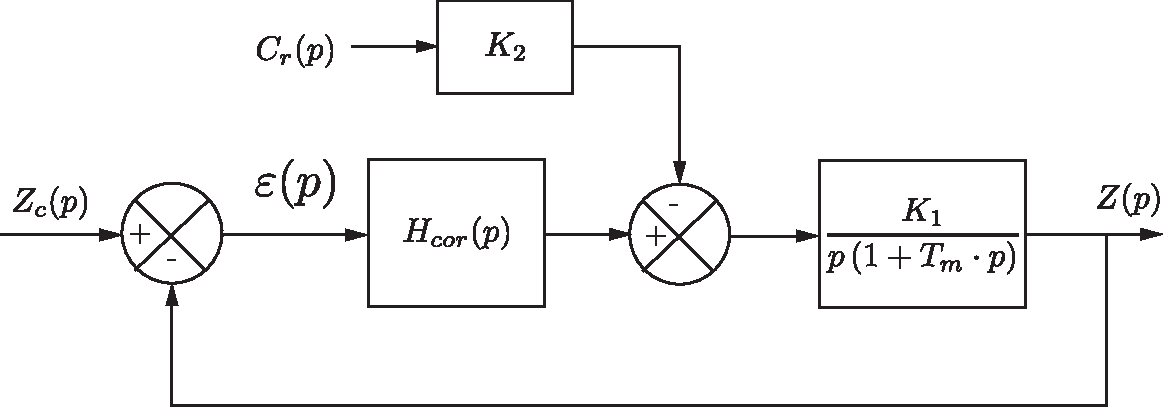
\includegraphics[width=\linewidth]{64_01}
\end{marginfigure}

\fi

 
\question{En considérant le retard nul, déterminer l'écart statique.}
\ifprof

La boucle fermée est de gain unitaire. On a donc $\varepsilon_S = 0$.
\else 
\fi

\question{En considérant le retard nul, déterminer l'expression de la boucle ouverte $H_{\text{BO}}(p)$.}
\ifprof

On a $G(p)=\dfrac{F(p)}{1+F(p)}$ avec $F(p)$ la FTBO. On donc $G(p)+G(p)F(p)=F(p)$ et
 $F(p)=\dfrac{G(p)}{1-G(p)} $
 $ = \dfrac{\dfrac{3,24}{p^2+3,24 p+3,24}}{1-\dfrac{3,24}{p^2+3,24 p+3,24}} $
  $ = \dfrac{3,24}{p\left(p+3,24\right)} $. 

\else 
\fi
 
\question{Déterminer l'expression de $G_r(p)$, transmittance en boucle fermée du système avec retard de \SI{0,2}{s}.}
\ifprof

On a $G_r(p)=\dfrac{\indice{H}{BO}(p)e^{-0,2 p}}{1+\indice{H}{BO}(p)e^{-0,2 p}}$ 
$=\dfrac{\dfrac{3,24}{p\left(p+3,24\right)}e^{-0,2 p}}{1+\dfrac{3,24}{p\left(p+3,24\right)}e^{-0,2 p}}$
$=\dfrac{3,24e^{-0,2 p}}{p\left(p+3,24\right)+3,24e^{-0,2 p}}$.
\else 
\fi

Le système est soumis à une rampe de \SI{0,1}{rad.s^{-1}}.
 
\question{Donner la valeur de l’erreur de traînage correspondant à cette entrée, en
négligeant le retard.}
\ifprof

On a $\lim\limits_{t\to +\infty} \varepsilon(t) $
$= \lim\limits_{p\to 0} p\varepsilon(p) $
$= \lim\limits_{p\to 0} p\left( \Theta_C(p) - \Theta_S(p) \right) $
$= \lim\limits_{p\to 0} p\left( \dfrac{0,1}{p^2}-\dfrac{0,1}{p^2} G_r(p) \right) $
$= \lim\limits_{p\to 0}  \dfrac{0,1}{p}\left(1-\dfrac{3,24e^{-0,2 p}}{p\left(p+3,24\right)+3,24e^{-0,2 p}} \right) $
$= \lim\limits_{p\to 0}  \dfrac{0,1}{p}\dfrac{p\left(p+3,24\right)+3,24e^{-0,2 p}-3,24e^{-0,2 p}}{p\left(p+3,24\right)+3,24e^{-0,2 p}}  $
$= \lim\limits_{p\to 0}  \dfrac{0,1}{p}\dfrac{p\left(p+3,24\right)}{p\left(p+3,24\right)+3,24e^{-0,2 p}}  $
$= \lim\limits_{p\to 0}  0,1\dfrac{\left(p+3,24\right)}{p\left(p+3,24\right)+3,24e^{-0,2 p}}  $
$=  0,1 $
\else 
\fi
 
\question{Donner la valeur de l'écart statique du système avec retard.}
\ifprof
\else 
\fi
 
\question{Donner la valeur de l'erreur de traînage du système avec retard.}
\ifprof
\else 
\fi

\ifprof
\else

\noindent\footnotesize
% \fbox{\parbox{.9\linewidth}{
% Éléments de corrigé : 
% \begin{enumerate}
  % \item $\varepsilon_{\text{con \%}} = \dfrac{1}{1+K_PK_m K_{\text{pom}} K_{\text{cap}} }$;
  % \item $K_P > 19$;
  % \item $\varepsilon_{\text{pert}} = \Delta Q_e \dfrac{K_f}{1+K_{\text{cap}}K_PK_mK_{\text{pom}}}$;
  % \item $K_P > 2,19$.
  % \item $K_P < 0,125$. Il est impossible de vérifier les trois conditions avec un correcteur proportionnel.
% \end{enumerate}}}
\normalsize


\marginnote{Corrigé voir \ref{PERF:06:C2:03:prec:64}.}

\fi 
 
\graphicspath{{\repStyle/png/}{../PERF/PERF-06-Precision/73_Bassin/images/}} 
\normaltrue \difficilefalse \tdifficilefalse
\correctionfalse
%\UPSTIidClasse{11} % 11 sup, 12 spé
%\newcommand{\UPSTIidClasse}{11}

\exer{ $\star$ \label{C2:03:prec:73}}
%% CCP MP 2007
\setcounter{question}{0}\UPSTIcompetence[2]{C2-03}
\index{Compétence C2-03}
\index{Schéma-blocs}
\index{Précision}

\ifcorrection
\else
\marginnote{\textbf{Pas de corrigé pour cet exercice.}}
\fi


\ifprof
\else
L'asservissement de vitesse est à présent modélisé par le schéma-blocs de la figure suivante à retour unitaire. Cet asservissement n’est valable que pour les petites variations de vitesse. $H(p)$ correspond à la fonction de transfert en boucle ouverte naturelle (non corrigée), $C(p)$ est le correcteur.

\begin{center}
\includegraphics[width=.7\linewidth]{73_01}
\end{center}

 $H(p)=\dfrac{K_N}{(1+T_m p)(1+T_e p)}$ avec $K_N = \SI{20}{ms.^{-1}V^{-1}}$, $T_m = \SI{5}{s}$, $T_e = \SI{0,5}{s}$.
 
 \begin{obj}
\begin{itemize}
\item  Exigence 1.2 : Garantir un déplacement du chariot de vitesse : 
\begin{itemize}
\item  1.2.3 Précision :
\begin{itemize}
\item Erreur statique pour une entrée $v_c(t)=V_0 u(t)$ avec $V_0 = \SI{8}{m.s^{-1}}$ : $E_S = \SI{0}{m.s^{-1}}$.
\item Erreur de trainage pour une entrée $v_c(t)=\gamma_0 t  u(t)$ avec $\gamma_0 = \SI{1,6}{m.s^{-2}}$ : $E_T \leq   \SI{0,16}{m.s^{-1}}$.
\end{itemize}
\end{itemize}
\end{itemize}
 \end{obj}
 Le concepteur choisit un correcteur Proportionnel Intégral : $C_1(p)=\dfrac{C}{T_i p} \left(1+T_i p\right)$ avec $T_i = T_m$.
 
\fi
 
 
\question{Déterminer les expressions littérales de l'erreur statique $E_S$ (consigne : échelon d'amplitude $V_0$) et de l'erreur de trainage $E_T$ (consigne : rampe de pente $\gamma_0$) de cet asservissement corrigé avec $C_1(p)$ en fonction de la consigne, du gain $K_N$ et des paramètres du correcteur et $C$  et $T_m$.}
\ifprof
\else 
\fi

\question{ En déduire la condition (notée $C_{\varepsilon}$) sur le gain $C$ du correcteur permettant de satisfaire l’exigence 1.2.3 du cahier des charges.}
\ifprof
\else 
\fi

On choisit finalement un correcteur PID : $C_2(p)=C\left(1+\dfrac{1}{T_i p}+T_d p \right)$ avec $T_i = 2 T_e$ et $T_d = \dfrac{T_e}{2}$.

\question{Montrer qu'on peut mettre ce correcteur sous la forme  $C_2(p)= \dfrac{K}{p}\left(1+Tp\right)^2$ et donner les expressions de $K$  et de $T$ en fonction de $C$ et $T_e$.}
\ifprof
\else 
\fi


\question{Donner l'expression de la fonction de transfert en boucle ouverte du système corrigé.}
\ifprof
\else 
\fi

\question{Déterminer les expressions littérales de l'erreur statique $E_S$ (consigne : échelon d'amplitude $V_0$) et de l'erreur de trainage $E_T$ (consigne : rampe de pente $\gamma_0$) de cet asservissement corrigé.}
\ifprof
\else 
\fi

\question{ En déduire la condition sur la valeur du gain $K$ du correcteur permettant de satisfaire l’exigence 1.2.3 du cahier des charges.}
\ifprof
\else 
\fi

\ifprof
\else

\noindent\footnotesize
% \fbox{\parbox{.9\linewidth}{
% Éléments de corrigé : 
% \begin{enumerate}
  % \item $\varepsilon_{\text{con \%}} = \dfrac{1}{1+K_PK_m K_{\text{pom}} K_{\text{cap}} }$;
  % \item $K_P > 19$;
  % \item $\varepsilon_{\text{pert}} = \Delta Q_e \dfrac{K_f}{1+K_{\text{cap}}K_PK_mK_{\text{pom}}}$;
  % \item $K_P > 2,19$.
  % \item $K_P < 0,125$. Il est impossible de vérifier les trois conditions avec un correcteur proportionnel.
% \end{enumerate}}}
\normalsize

\begin{flushright}
\footnotesize{Corrigé  voir \ref{C2:03:prec:73}.}
\end{flushright}%
\fi 
 
